% Capítulo 3 – gerado a partir do relatório; edite livremente
\chapter{PLANO DE TRABALHO}

\section{Sequência de operações}

A sequência adotada está resumida na Figura~\ref{fig:roteiro}. O torneamento é feito em duas fixações (operações 20 e 30) e gera todas as superfícies de revolução, inclusive o furo, que é aberto com broca e mandrilado no próprio torno. Em seguida vêm o fresamento dos dentes, o fresamento dos rasgos em arco e o brochamento do rasgo de chaveta, ainda com o material recozido. Depois da rebarbação e do tratamento térmico, as faces do cubo e o furo são retificados. Ao todo são empregados cinco processos de usinagem: torneamento, furação, fresamento, brochamento e retificação.


\begin{figure}[H]
\centering
\caption{Sequência de fabricação da engrenagem}\label{fig:roteiro}
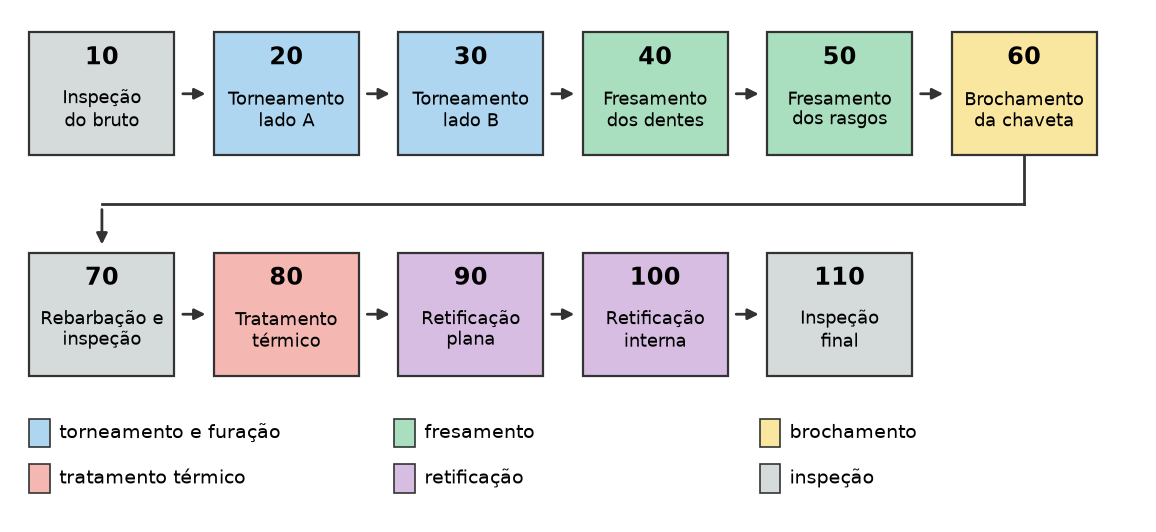
\includegraphics[width=15cm]{figuras/fig_roteiro.png}
\fonte{Elaborado pelos autores.}
\end{figure}


Para os dentes foram consideradas duas alternativas: o fresamento com fresa de disco de perfil evolvente, em fresadora universal com cabeçote divisor, e a geração com fresa caracol em fresadora de engrenagens. Escolheu-se a primeira porque utiliza uma máquina comum em ferramentarias e laboratórios, é adequada a lotes pequenos e corresponde ao fresamento tangencial estudado nas Aulas 15 a 17. A fresa caracol, comparada na Seção 3.4, seria a opção para produção seriada.


\section{Referências e fixação}

A face A do cubo e o furo, usinados na mesma fixação da operação 20, são as referências de todo o processo. Na operação 30 a peça é presa pelo Ø156 já torneado, em castanhas moles usinadas no próprio torno, e apoiada pela face A em um anel de encosto, o que garante o paralelismo entre as faces do cubo. Nas operações 40, 50 e 60 a peça é localizada pelo furo, com mandril ou pino, e pela face A. Depois do tratamento térmico, as faces do cubo são retificadas apoiando-se uma na outra e, por último, o furo é retificado com a peça centrada pelo diâmetro primitivo dos dentes, em uma placa com roletes alojados entre os dentes. Desse modo, o furo final fica concêntrico ao dentado, que é o requisito funcional mais importante da engrenagem.


\section{Descrição das operações}

\subsection*{Operação 10 – Inspeção do bruto}
\addcontentsline{toc}{subsection}{Operação 10 – Inspeção do bruto}

A barra serrada é conferida quanto ao diâmetro, ao comprimento e à dureza, e o certificado do material é verificado. São usados paquímetro e durômetro, na bancada (Figura~\ref{fig:op10}).


\begin{figure}[H]
\centering
\caption{Operação 10 – bruto serrado}\label{fig:op10}
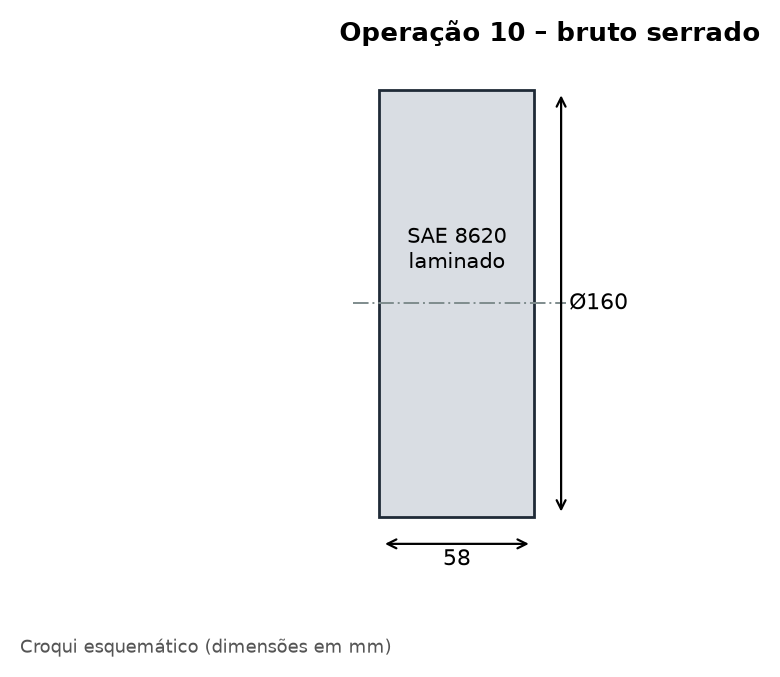
\includegraphics[width=6cm]{figuras/croqui_op10.png}
\fonte{Elaborado pelos autores.}
\end{figure}


\subsection*{Operação 20 – Torneamento do lado A}
\addcontentsline{toc}{subsection}{Operação 20 – Torneamento do lado A}

A peça é presa pelo diâmetro bruto em placa de três castanhas duras, com 15 mm de pega, no torno CNC ROMI Centur 30D. A face A é faceada em dois passes de desbaste de 1,425 mm e um passe de acabamento de 0,5 mm, que deixa 0,15 mm para a retificação da face do cubo. Em seguida, o diâmetro externo é desbastado de Ø160 para Ø157 ao longo de 36 mm e a face do aro é rebaixada 1,65 mm em relação à face do cubo, formando o ressalto do cubo (Figura~\ref{fig:op20a}). O passe de acabamento, com outra ferramenta, percorre o contorno da face do cubo, o Ø46 com o chanfro de 2 mm, a face do aro e o Ø156.


\begin{figure}[H]
\centering
\caption{Operação 20 – faceamento, torneamento externo e degrau do aro}\label{fig:op20a}
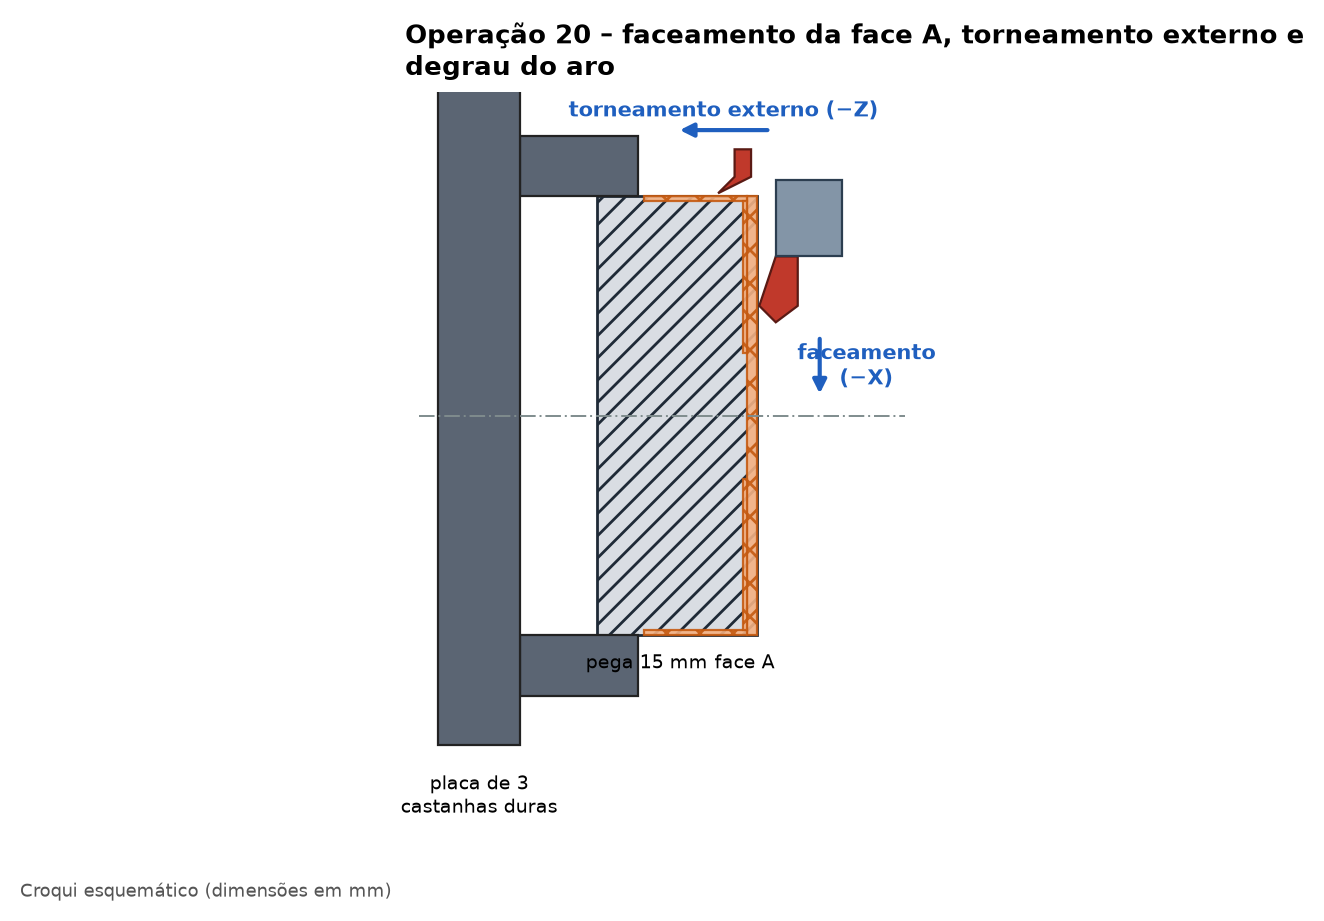
\includegraphics[width=11cm]{figuras/croqui_op20a.png}
\fonte{Elaborado pelos autores.}
\end{figure}


Sem soltar a peça, o furo é aberto com broca de Ø23 mm, passante, e mandrilado para Ø24,5 mm, o que deixa 0,25 mm no raio para a retificação interna (Figura~\ref{fig:op20b}). Por fim, o rebaixo da face A, entre Ø46 e Ø110 e com 17 mm de profundidade a partir da face do aro, é usinado com ferramenta de canal frontal: oito mergulhos axiais, do diâmetro maior para o menor e com passo radial de 4 mm, seguidos de um passe de contorno que acaba as paredes, o fundo e os raios de 3 mm (Figura~\ref{fig:op20c}). As arestas são quebradas com 0,5 $\times$ 45°. Em todas as etapas usa-se emulsão de óleo solúvel como fluido de corte.


\begin{figure}[H]
\centering
\caption{Operação 20 – furação e mandrilamento}\label{fig:op20b}
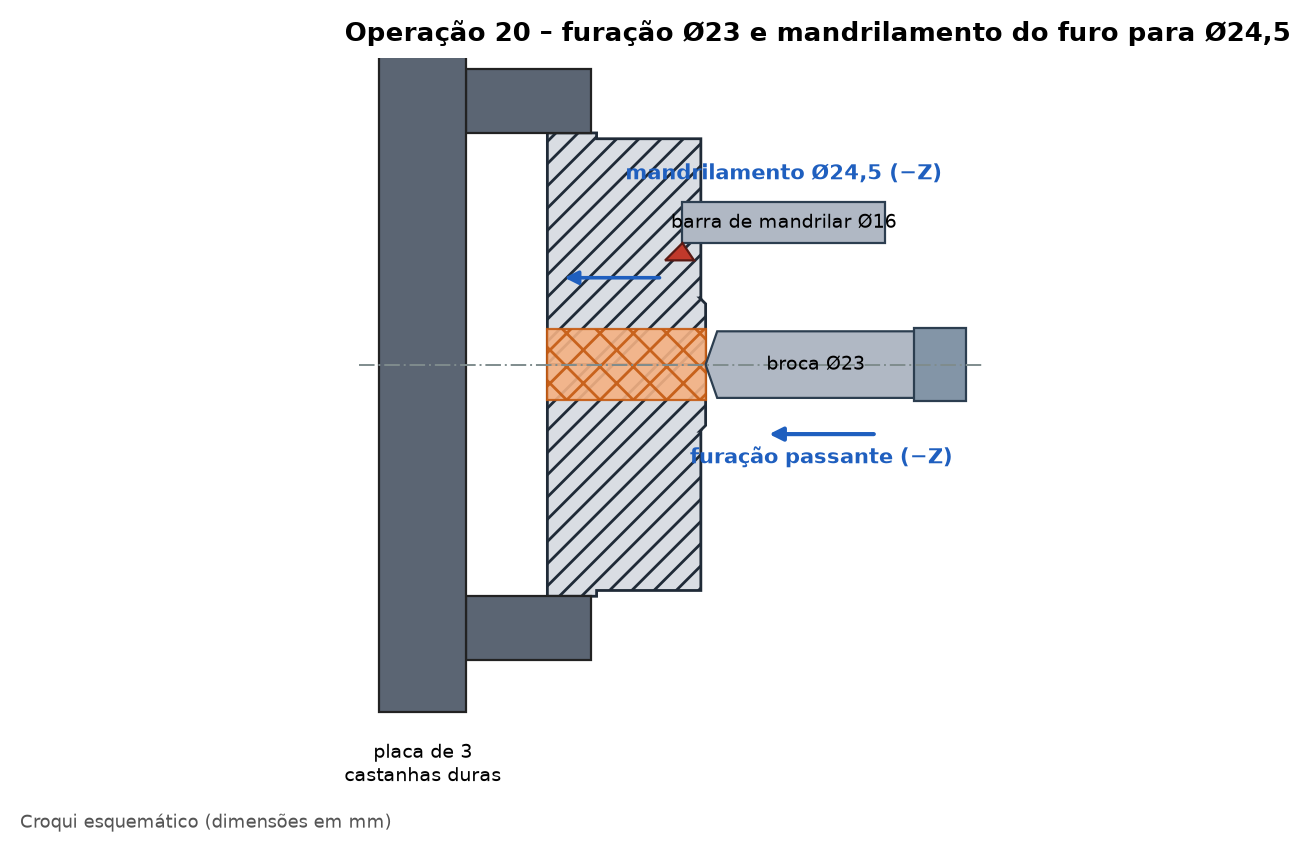
\includegraphics[width=11cm]{figuras/croqui_op20b.png}
\fonte{Elaborado pelos autores.}
\end{figure}


\begin{figure}[H]
\centering
\caption{Operação 20 – rebaixo frontal da face A}\label{fig:op20c}
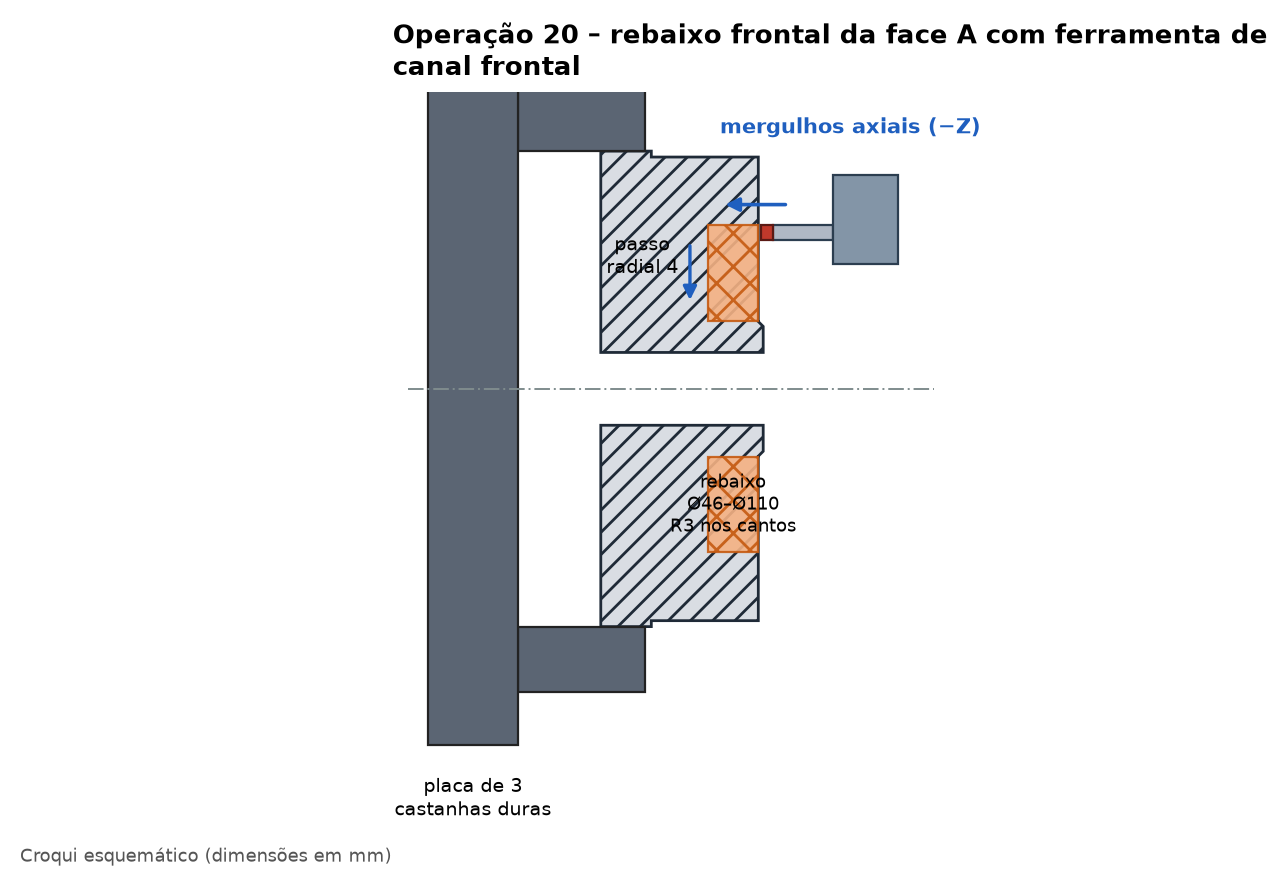
\includegraphics[width=11cm]{figuras/croqui_op20c.png}
\fonte{Elaborado pelos autores.}
\end{figure}


\subsection*{Operação 30 – Torneamento do lado B}
\addcontentsline{toc}{subsection}{Operação 30 – Torneamento do lado B}

A peça é invertida e presa pelo Ø156 em castanhas moles usinadas no próprio torno, com a face A do cubo apoiada em um anel de encosto (Figura~\ref{fig:op30}). Repetem-se o faceamento, agora até o comprimento de 51,3 mm no cubo, o torneamento dos 16 mm do Ø156 que estavam sob as castanhas na operação anterior, o degrau do aro, o acabamento e o rebaixo da face B, com as mesmas ferramentas e parâmetros da operação 20.


\begin{figure}[H]
\centering
\caption{Operação 30 – torneamento do lado B}\label{fig:op30}
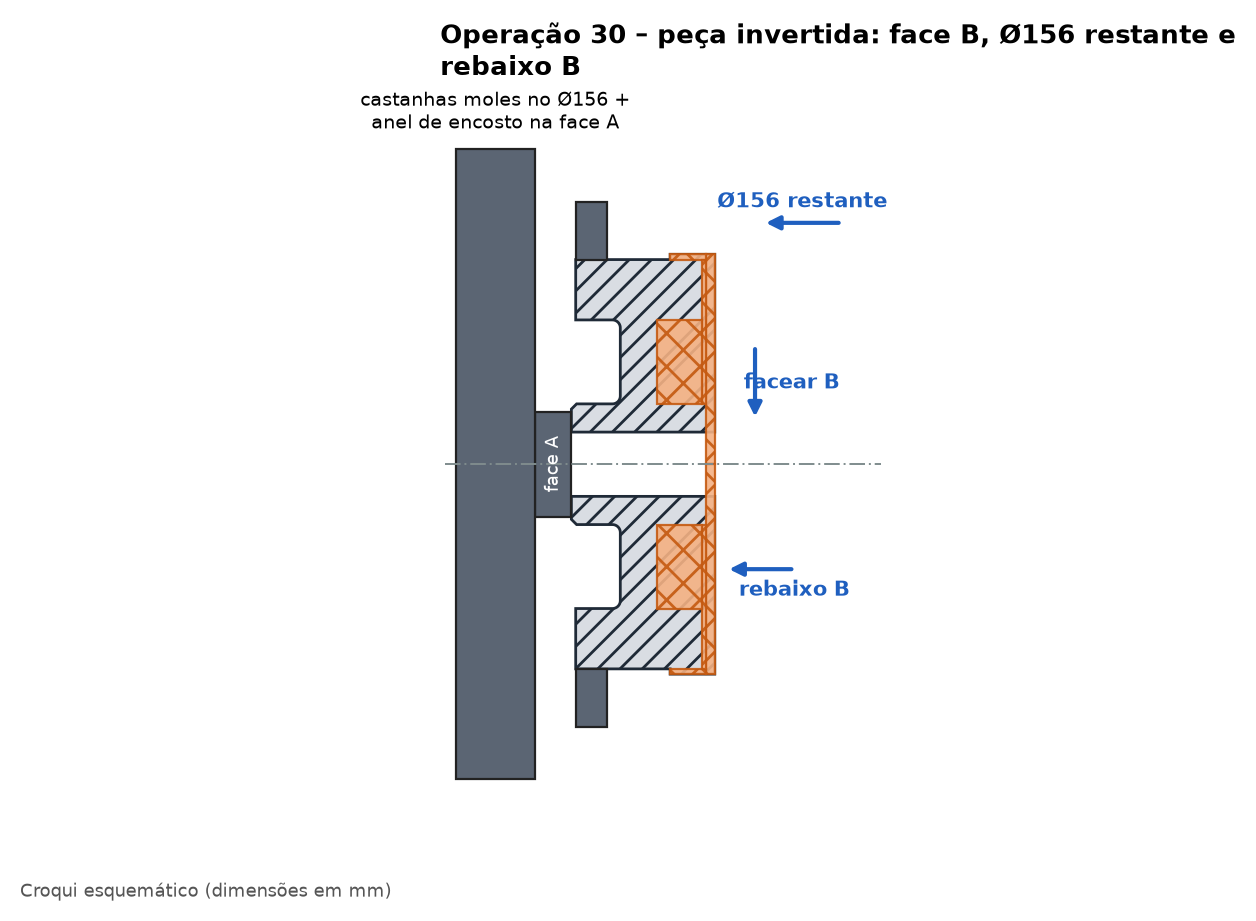
\includegraphics[width=11cm]{figuras/croqui_op30.png}
\fonte{Elaborado pelos autores.}
\end{figure}


\subsection*{Operação 40 – Fresamento dos dentes}
\addcontentsline{toc}{subsection}{Operação 40 – Fresamento dos dentes}

A peça é montada em um mandril de Ø24,5 mm, encostada pela face A e presa por porca, entre o cabeçote divisor e a contraponta da fresadora universal KNUTH UWF 5 (Figura~\ref{fig:op40}). A fresa de disco de módulo 6 nº 4, que atende engrenagens de 21 a 25 dentes, é centrada em relação ao eixo da peça, e cada vão é fresado com o avanço da mesa paralelo a esse eixo. Primeiro todos os vãos são desbastados com profundidade de 12,6 mm (2,1 vezes o módulo, conforme o fabricante da fresa) e depois todos são acabados na altura total do dente, 13 mm. Entre um vão e o seguinte o cabeçote divisor gira a peça de 15°, o que, com a relação de 40:1, corresponde a uma volta da manivela mais 12 furos no disco de 18 furos. O fluido é óleo integral, indicado para o corte de dentes de engrenagem.


\begin{figure}[H]
\centering
\caption{Operação 40 – fresamento dos dentes}\label{fig:op40}
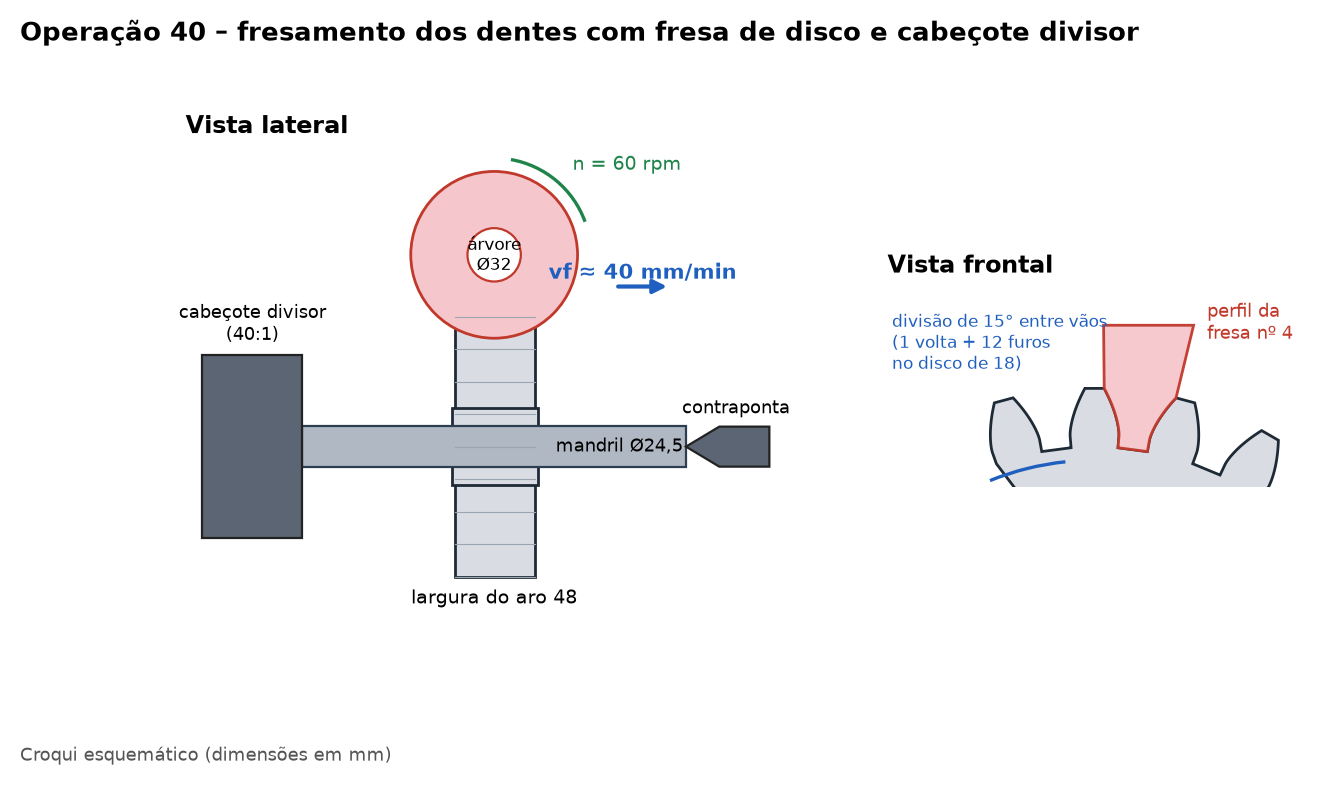
\includegraphics[width=15cm]{figuras/croqui_op40.png}
\fonte{Elaborado pelos autores.}
\end{figure}


\subsection*{Operação 50 – Fresamento dos rasgos em arco}
\addcontentsline{toc}{subsection}{Operação 50 – Fresamento dos rasgos em arco}

No centro de usinagem vertical ROMI D 800, a peça é centrada por um pino de Ø24,5 mm, apoiada pela face do cubo em uma placa-base e presa por porca e arruela (Figura~\ref{fig:op50}). Cada rasgo é aberto com fresa de topo de Ø16 mm: a fresa entra em rampa de 5° ao longo da linha de centro, de raio 39 mm, desbasta em três níveis de até 5 mm até atravessar a alma e, por último, faz um contorno de acabamento com 1 mm de penetração lateral, que leva a largura do rasgo a 18 mm e forma as extremidades de raio 9 mm. A usinagem é feita a seco, com ar comprimido para retirar os cavacos do rasgo.


\begin{figure}[H]
\centering
\caption{Operação 50 – fresamento dos rasgos em arco}\label{fig:op50}
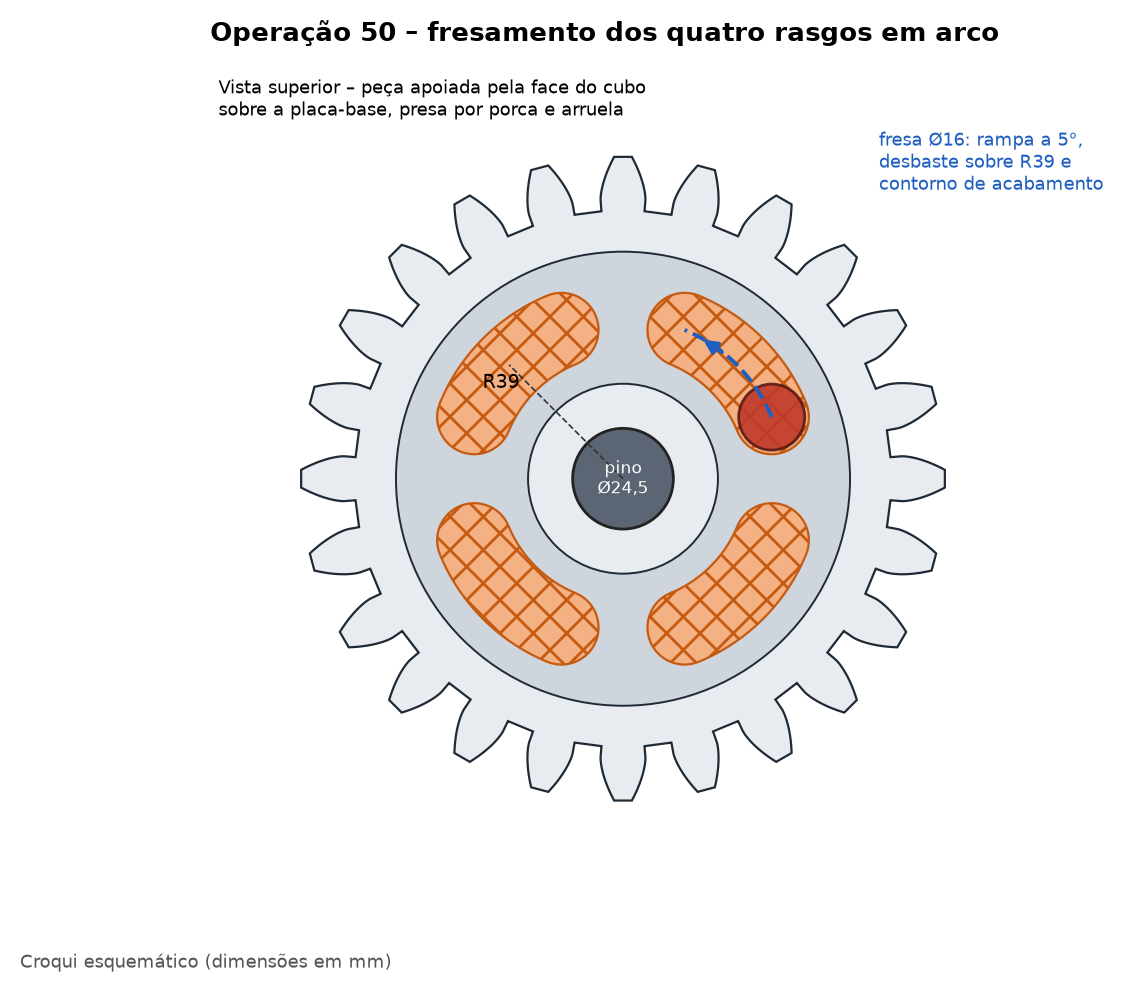
\includegraphics[width=9.5cm]{figuras/croqui_op50.png}
\fonte{Elaborado pelos autores.}
\end{figure}


\subsection*{Operação 60 – Brochamento do rasgo de chaveta}
\addcontentsline{toc}{subsection}{Operação 60 – Brochamento do rasgo de chaveta}

O rasgo de 8 mm é brochado em prensa hidráulica, com a brocha guiada por uma bucha de Ø24,5 mm encaixada no furo (Figura~\ref{fig:op60}). A peça apoia-se pela face A em um suporte com um pino que entra em um dos rasgos em arco, para que a chaveta fique simétrica em relação a eles. São necessários dois passes, o segundo com calço, até que o fundo do rasgo fique a 16 mm do eixo do furo (28,5 mm até a geratriz oposta do furo acabado). Como essa cota é referida ao eixo, ela não se altera quando o furo for retificado para Ø25. Usa-se óleo integral de alta viscosidade.


\begin{figure}[H]
\centering
\caption{Operação 60 – brochamento do rasgo de chaveta}\label{fig:op60}
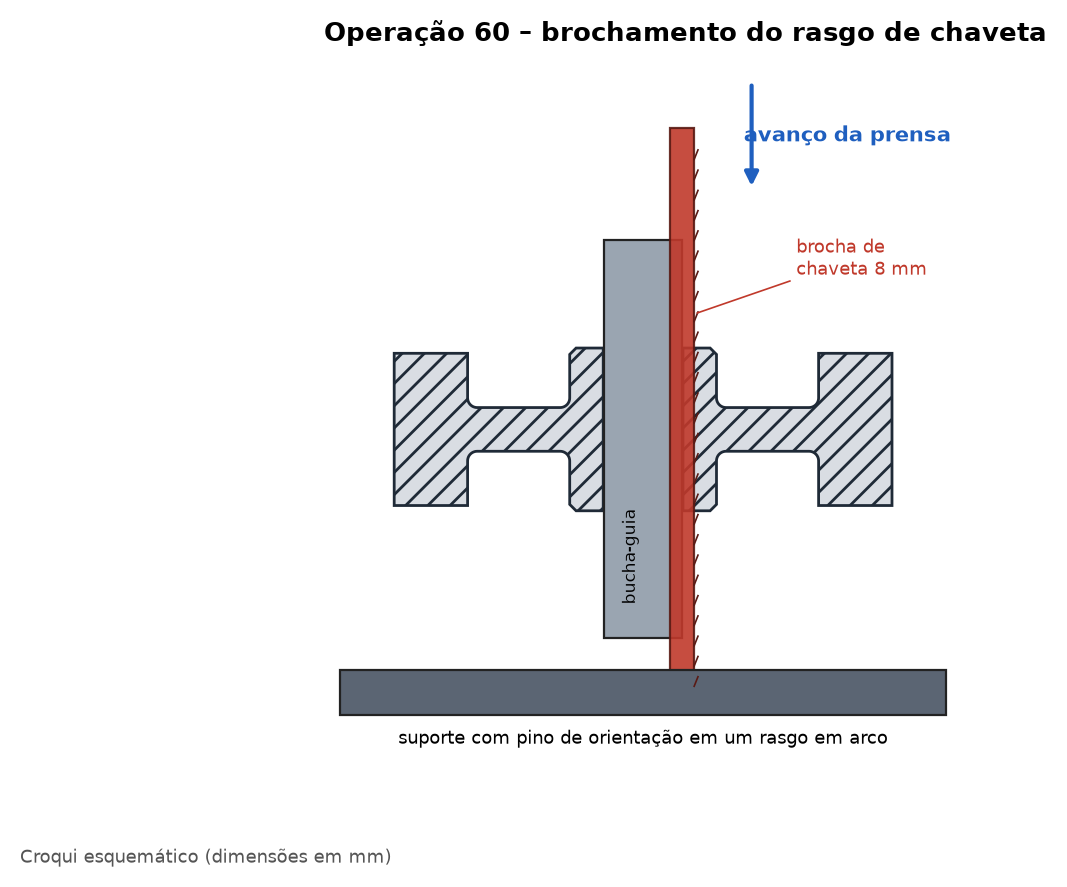
\includegraphics[width=9.5cm]{figuras/croqui_op60.png}
\fonte{Elaborado pelos autores.}
\end{figure}


\subsection*{Operação 70 – Rebarbação e inspeção intermediária}
\addcontentsline{toc}{subsection}{Operação 70 – Rebarbação e inspeção intermediária}

As rebarbas dos dentes, dos rasgos e da chaveta são removidas na bancada, e a espessura dos dentes é conferida pela medida sobre 3 dentes com micrômetro de pratos (Figura~\ref{fig:op110}), cujo valor nominal é 46,30 mm. É a última verificação antes do tratamento térmico, enquanto a peça ainda pode ser corrigida.


\begin{figure}[H]
\centering
\caption{Medição sobre 3 dentes com micrômetro de pratos}\label{fig:op110}
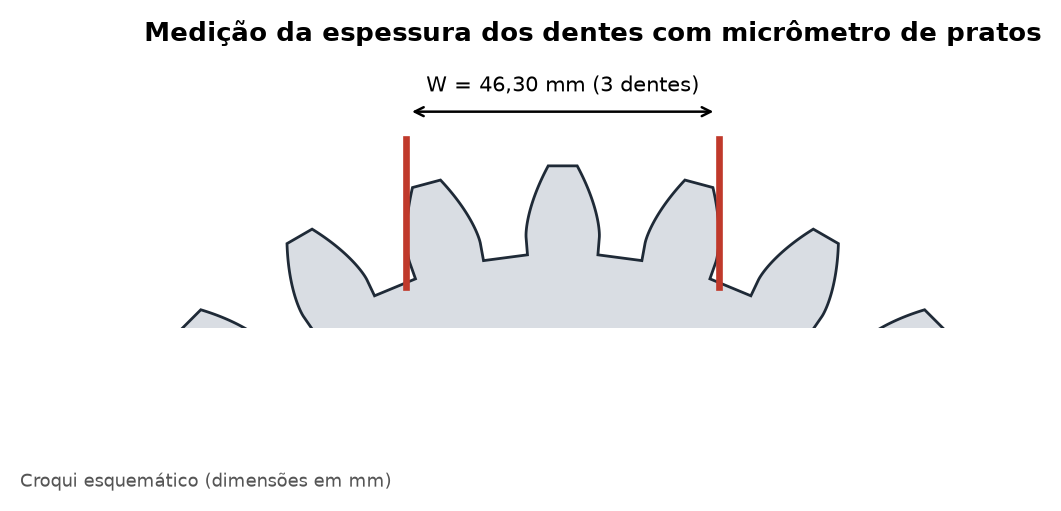
\includegraphics[width=8cm]{figuras/croqui_op110.png}
\fonte{Elaborado pelos autores.}
\end{figure}


\subsection*{Operação 80 – Tratamento térmico}
\addcontentsline{toc}{subsection}{Operação 80 – Tratamento térmico}

A cementação, a têmpera e o revenimento são executados por fornecedor especializado, conforme o Quadro~\ref{quad:espec}.


\subsection*{Operação 90 – Retificação plana das faces do cubo}
\addcontentsline{toc}{subsection}{Operação 90 – Retificação plana das faces do cubo}

Na retificadora plana KNUTH HFS 3063 F Advance, a peça é colocada sobre a mesa magnética apoiada por uma das faces do cubo, e a face oposta é retificada; depois a peça é invertida e a outra face é levada ao comprimento de 51,00 mm (Figura~\ref{fig:op90}). Como o cubo sobressai 1,5 mm do aro, somente as faces do cubo tocam o rebolo. São dados passes de desbaste de 0,02 mm, passes de acabamento de 0,005 mm e dois passes sem penetração (faiscamento), com refrigeração abundante. Ao final, a peça é desmagnetizada.


\begin{figure}[H]
\centering
\caption{Operação 90 – retificação plana das faces do cubo}\label{fig:op90}
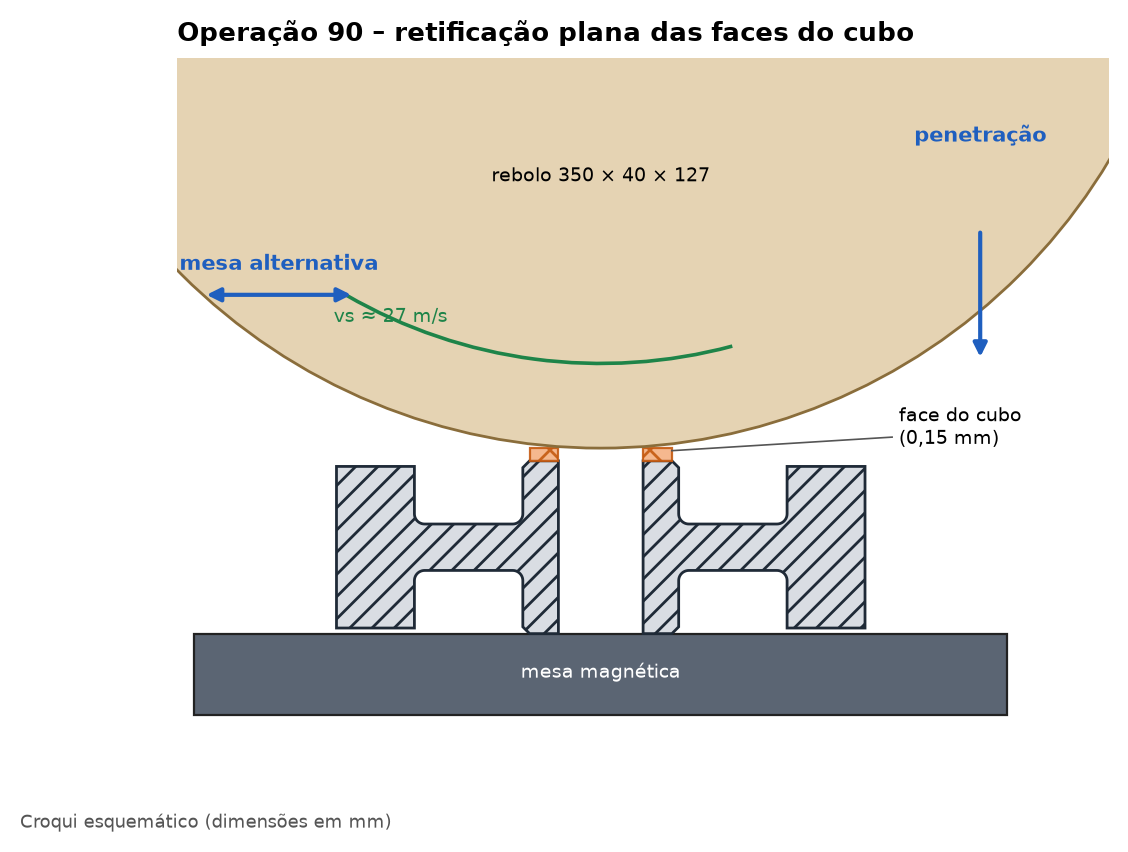
\includegraphics[width=10cm]{figuras/croqui_op90.png}
\fonte{Elaborado pelos autores.}
\end{figure}


\subsection*{Operação 100 – Retificação interna do furo}
\addcontentsline{toc}{subsection}{Operação 100 – Retificação interna do furo}

Na retificadora interna STUDER S121, a peça é centrada pelo diâmetro primitivo em uma placa com três roletes calibrados alojados entre os dentes e apoiada pela face A já retificada (Figura~\ref{fig:op100}). O furo é retificado de Ø24,5 para Ø25 H7 com rebolo de Ø20 mm, em retificação de passagem com oscilação axial, terminando com passes de faiscamento.


\begin{figure}[H]
\centering
\caption{Operação 100 – retificação interna do furo}\label{fig:op100}
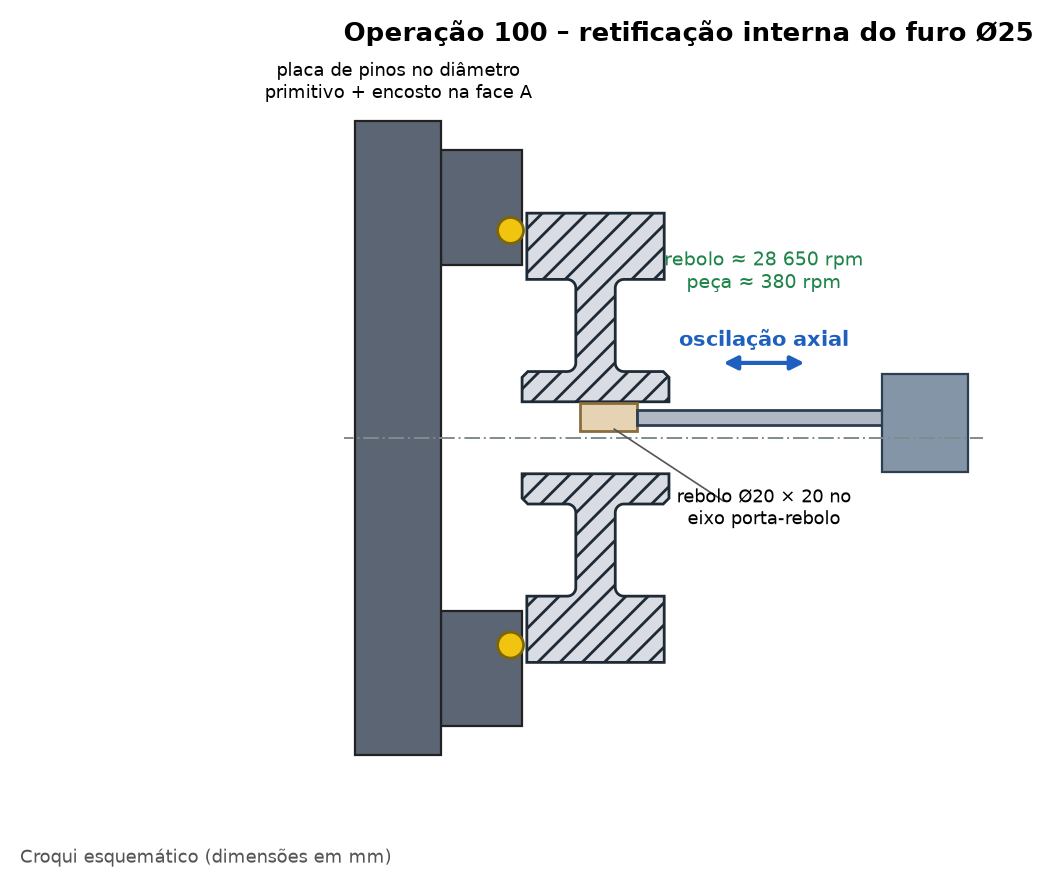
\includegraphics[width=10.5cm]{figuras/croqui_op100.png}
\fonte{Elaborado pelos autores.}
\end{figure}


\subsection*{Operação 110 – Inspeção final}
\addcontentsline{toc}{subsection}{Operação 110 – Inspeção final}

São verificados o furo (calibrador tampão), o comprimento do cubo, a medida sobre 3 dentes, o batimento do dentado em relação ao furo, a dureza superficial e a rugosidade das superfícies retificadas.


\section{Comparação com a geração por fresa caracol}

Na fresadora de engrenagens LIEBHERR LC 180, que aceita peças de até 180 mm de diâmetro e módulo até 6, uma fresa caracol de Ø100 mm trabalhando a 120 m/min, com avanço axial de 2,5 mm por volta da peça, cortaria os 24 dentes em cerca de 2 minutos, contra 105 minutos do fresamento com fresa de disco. Além disso, o perfil gerado é exato para qualquer número de dentes, enquanto a fresa de disco nº 4 tem o perfil exato apenas para 21 dentes. Para um lote pequeno, entretanto, o custo da fresa caracol e da máquina dedicada não se justifica, e o fresamento com fresa de disco atende à qualidade adotada para os dentes.

